\documentclass[../main.tex]{subfiles} 

\renewcommand{\imageSrc}{../images/}

\begin{document}
\chapter{Introduction}

\section{Classification}

The table below shows how computing systems can be classified. Please note that a system can refer to a simple program or a whole computer system. A system can be classified by its response time requirements or by the need of external interaction. 

\begin{itemize}
	\item \textbf{Non Real-Time Data Processing} \\
	There is no external stimulation of the system, it justs processes data. There are no time constraints.
	\item \textbf{Real-Time Data Processing} \\
	The system is paced by their external environment. The response time constraints are twofold: teh \textbf{accept data} rate is dictated by the producer, the \textbf{processing rate} is dependent on the external environment.
	\item \textbf{Non Real-Time Reactive (Interactive)} \\
	Systems stimulated by the human user. The response time is expected to be as short as possible. The pace is set by the slowest entity: the user.
	\item \textbf{Real-Time Reactive} \\
	The external environment controls the system which processes data at peak rate.
\end{itemize}

Real-Time systems have a response time constraint. Usually this constraint is not really a timing constraint but rather an expression relative to a physical measurement unit.

\begin{exmp}
Take for example a carriage that must be stopped before it hits a bumper. The physical measurement unit here is \textbf{distance}. This constraint can easily be converted to a timing constraint given it's initial speak, braking characteristics etc. 
\begin{figure}[h!]
    \centering
    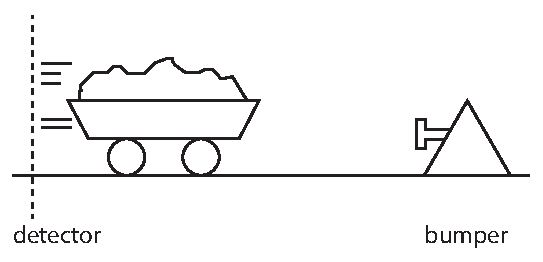
\includegraphics[width=0.4\textwidth]{\imageSrc/carriage.jpg}
    \caption{Example: Carriage stopping before bumper.}
    \label{eop}
\end{figure}
\end{exmp}

However, since a computer has no notion of distance, specifications in terms of physical units have to be converted to a timing constraint. When it comes to specifications on the other hand, it's better to include the original constraint than the computed timing constraint. This being sayd, the real-time programmer usually is only in charge of the computing system and cannot modify the original parameters.

Another way to classify real-time systems is by dividing them in \textbf{stand-alone systems} and systems that are \textbf{part of a hierarchy}. This course focusses on \textbf{embedded systems}: they are a component built-in to other equipment. They can either work alone or be part of a distributed system.

\begin{exmp}
An example of a \textbf{embedded system that works alone} is the electric ignition of a car, a modern washing machine or an electronic scale.
\end{exmp} 

\begin{exmp}
An example of a \textbf{embedded system that is part of a distributed system} is a network programmable controller, a programmable machine tool or more generally controllers dedicated to a component of a larger system.
\end{exmp} 


\section{Real-Time Architecture}
The classical architecture of a distributed real-time system is a two layer architecture:
\begin{enumerate}
	\item Dedicated System
	\item Coordinating systems
\end{enumerate}

\subsection{Dedicated Controllers}

\subsection{Central System}
\subsection{Connections}
\subsection{System Types}

\section{Time in a Real-Time System}

\section{Design Strategy}



\end{document}